%%%%%%%%%%%%%%%%%%%%%%%%%%%%%%%%%%%%%%%%%
% Beamer Presentation
% LaTeX Template
% Version 1.0 (10/11/12)
%
% This template has been downloaded from:
% http://www.LaTeXTemplates.com
%
% License:
% CC BY-NC-SA 3.0 (http://creativecommons.org/licenses/by-nc-sa/3.0/)
%
%%%%%%%%%%%%%%%%%%%%%%%%%%%%%%%%%%%%%%%%%

%----------------------------------------------------------------------------------------
%	PACKAGES AND THEMES
%----------------------------------------------------------------------------------------

\documentclass{beamer}

\mode<presentation> {

% The Beamer class comes with a number of default slide themes
% which change the colors and layouts of slides. Below this is a list
% of all the themes, uncomment each in turn to see what they look like.

%\usetheme{default}
%\usetheme{AnnArbor}
%\usetheme{Antibes}
%\usetheme{Bergen}
\usetheme{Berkeley}
%\usetheme{Berlin}
%\usetheme{Boadilla}
%\usetheme{CambridgeUS}
%\usetheme{Copenhagen}
%\usetheme{Darmstadt}
%\usetheme{Dresden}
%\usetheme{Frankfurt}
%\usetheme{Goettingen}
%\usetheme{Hannover}
%\usetheme{Ilmenau}
%\usetheme{JuanLesPins}
%\usetheme{Luebeck}
%\usetheme{Madrid}
%\usetheme{Malmoe}
%\usetheme{Marburg}
%\usetheme{Montpellier}
%\usetheme{PaloAlto}
%\usetheme{Pittsburgh}
%\usetheme{Rochester}
%\usetheme{Singapore}
%\usetheme{Szeged}
%\usetheme{Warsaw}

% As well as themes, the Beamer class has a number of color themes
% for any slide theme. Uncomment each of these in turn to see how it
% changes the colors of your current slide theme.

%\usecolortheme{albatross}
%\usecolortheme{beaver}
%\usecolortheme{beetle}
%\usecolortheme{crane}
%\usecolortheme{dolphin}
%\usecolortheme{fly}
%\usecolortheme{lily}
\usecolortheme{orchid}
%\usecolortheme{rose}
%\usecolortheme{seagull}
%\usecolortheme{seahorse}
%\usecolortheme{whale}
%\usecolortheme{wolverine}

%\setbeamertemplate{footline} % To remove the footer line in all slides uncomment this line
%\setbeamertemplate{footline}[page number] % To replace the footer line in all slides with a simple slide count uncomment this line

%\setbeamertemplate{navigation symbols}{} % To remove the navigation symbols from the bottom of all slides uncomment this line
}

\usepackage{graphicx} % Allows including images
\usepackage{booktabs} % Allows the use of \toprule, \midrule and \bottomrule in tables

\usepackage{listings}
\usepackage{color}
\usepackage{setspace}

\definecolor{mygray}{rgb}{0.4,0.4,0.4}
\definecolor{mygreen}{rgb}{0,0.8,0.6}
\definecolor{myorange}{rgb}{1.0,0.4,0}

\lstset{
basicstyle=\footnotesize\sffamily\color{black},
commentstyle=\color{mygray},
frame=single,
numbers=left,
numbersep=5pt,
numberstyle=\tiny\color{mygray},
keywordstyle=\color{mygreen},
showspaces=false,
showstringspaces=false,
stringstyle=\color{myorange},
tabsize=2
}


%---------------------------------------------------------------------------------------
%	TITLE PAGE
%----------------------------------------------------------------------------------------

\title{Comparison of dislocation fields} % The short title appears at the bottom of every slide, the full title is only on the title page

\author{Alex Olar} % Your name
\institute[ELTE] % Your institution as it will appear on the bottom of every slide, may be shorthand to save space
{
University of Eotvos Lorand \\ % Your institution for the title page
\medskip
\textit{olaralex@caesar.elte.hu} % Your email address
}
\date{\today} % Date, can be changed to a custom date

\begin{document}

\begin{frame}
    \titlepage % Print the title page as the first slide
\end{frame}

\begin{frame}
    \frametitle{The C++ code}

    \begin{center}
        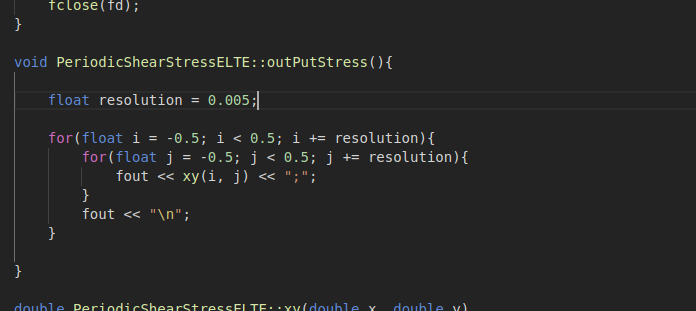
\includegraphics[width=.9\textwidth]{code.png}
    \end{center}

    \par Did not change.

\end{frame}

%----------------------------------------------------------------------------------------
%	PRESENTATION SLIDES

\begin{frame}
    \frametitle{Visualization, log scale}

    \par This changed heavily.

    \begin{center}
        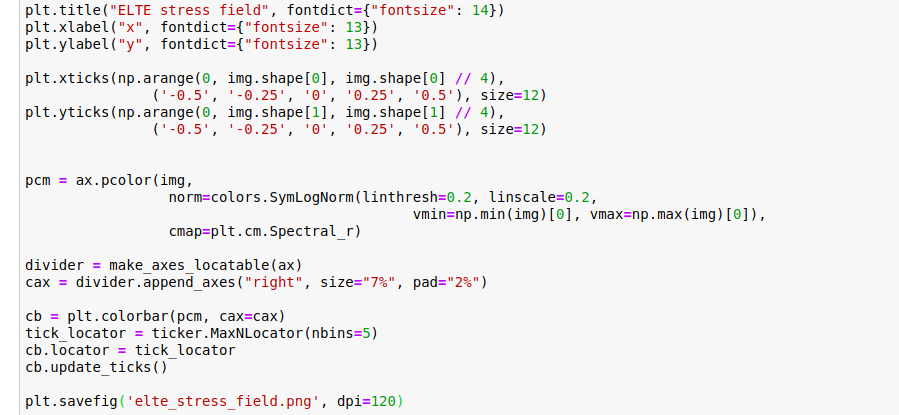
\includegraphics[width=.9\textwidth]{visu.png}
    \end{center}

\end{frame}

\begin{frame}
    \frametitle{Visualization, log scale}
    \par I used symmetric logarithmic scale with different thresholds
    based on the data. Therefore I could visualize negative and positive values
    with different, diverging colors.

    \vspace{1cm}

    \par That's the reason why the plots look so cool.
\end{frame}

%------------------------------------------------

\begin{frame}
    \frametitle{Plot 1}
    \begin{figure}[H]
        \centering
        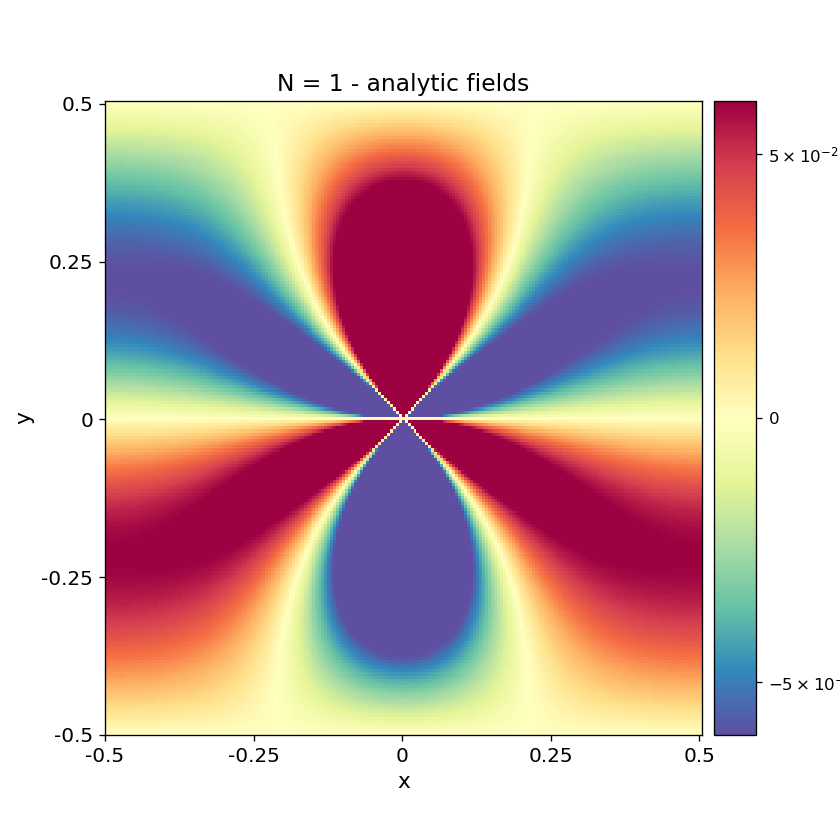
\includegraphics[width=0.7\textwidth]{../stress_field_01.png}
    \end{figure}
\end{frame}

\begin{frame}
    \frametitle{Plot 2}
    \begin{figure}[H]
        \centering
        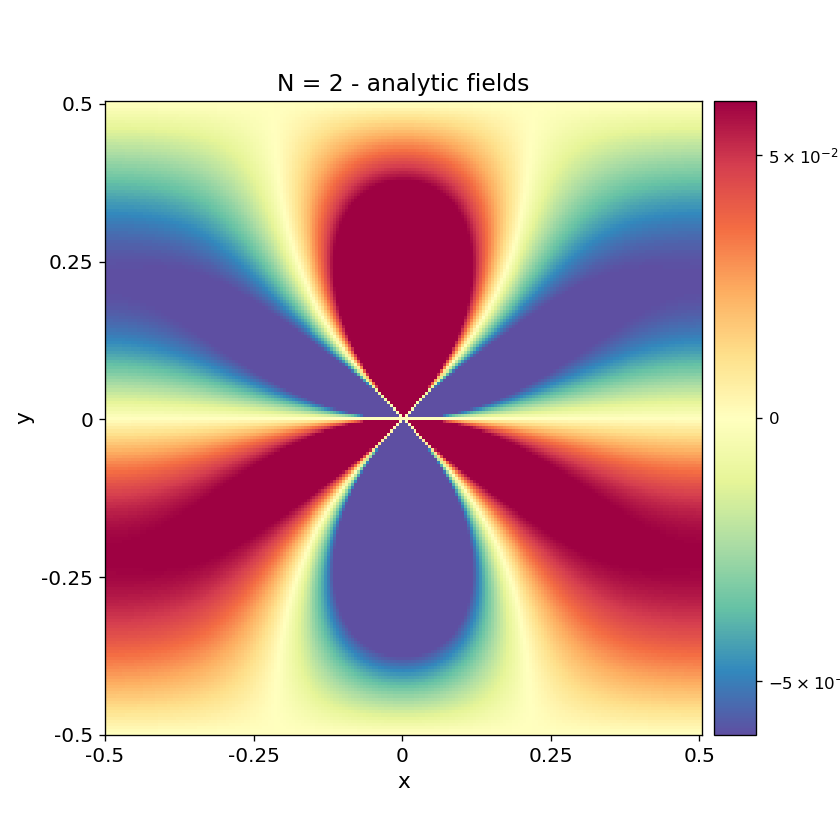
\includegraphics[width=0.7\textwidth]{../stress_field_02.png}
    \end{figure}
\end{frame}

\begin{frame}
    \frametitle{Plot 3}
    \begin{figure}[H]
        \centering
        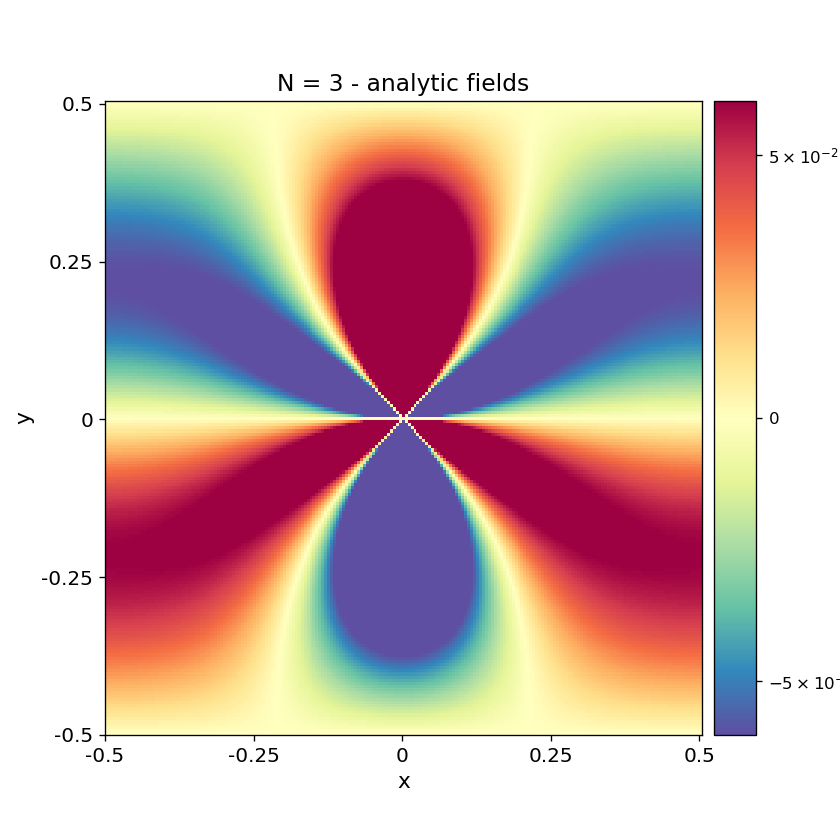
\includegraphics[width=0.7\textwidth]{../stress_field_03.png}
    \end{figure}
\end{frame}

\begin{frame}
    \frametitle{Plot 4}
    \begin{figure}[H]
        \centering
        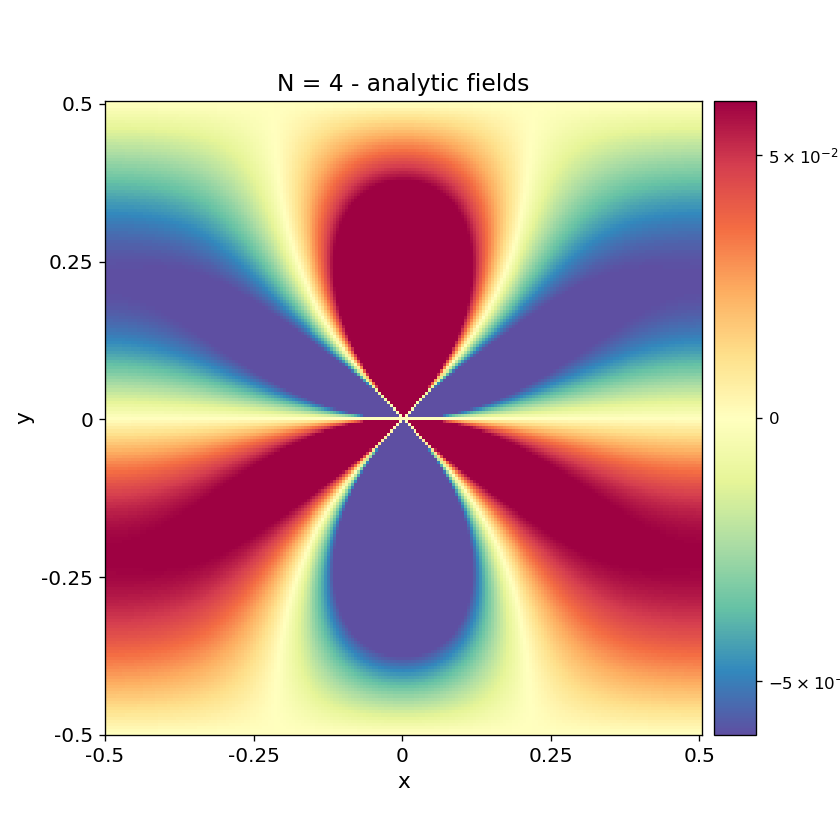
\includegraphics[width=0.7\textwidth]{../stress_field_04.png}
    \end{figure}
\end{frame}

\begin{frame}
    \frametitle{Plot 5}
    \begin{figure}[H]
        \centering
        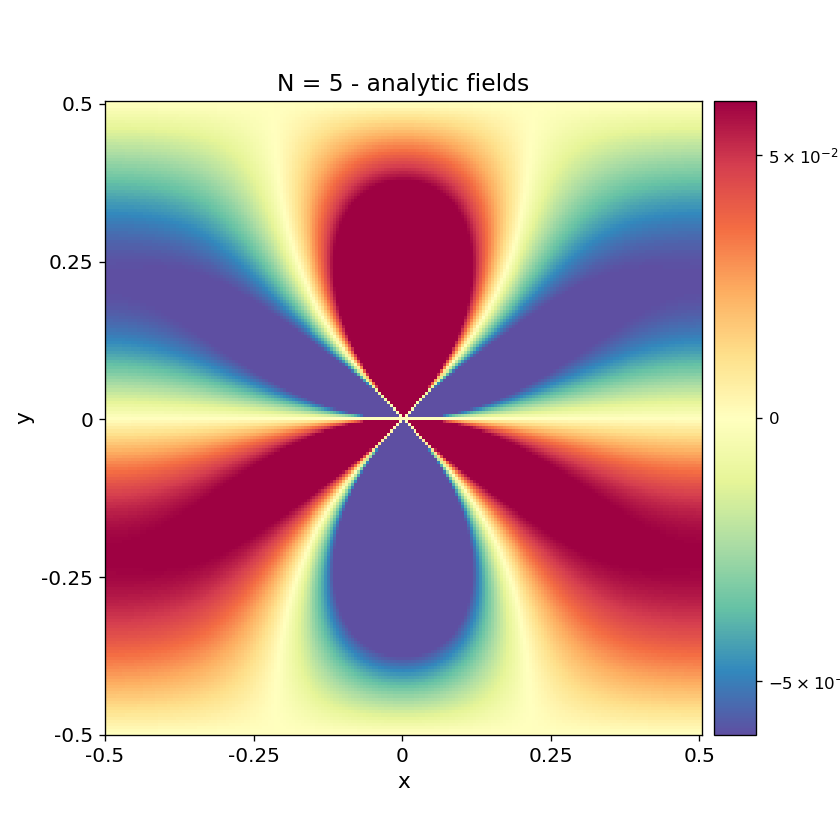
\includegraphics[width=0.7\textwidth]{../stress_field_05.png}
    \end{figure}
\end{frame}

\begin{frame}
    \frametitle{Plot 6}
    \begin{figure}[H]
        \centering
        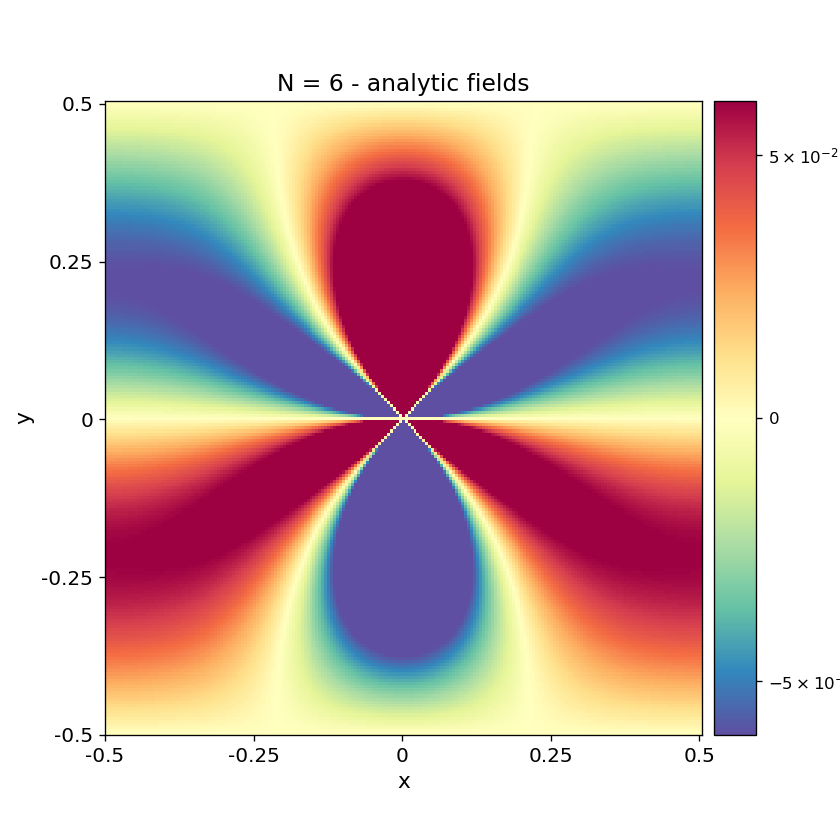
\includegraphics[width=0.7\textwidth]{../stress_field_06.png}
    \end{figure}
\end{frame}

\begin{frame}
    \frametitle{Plot 7}
    \begin{figure}[H]
        \centering
        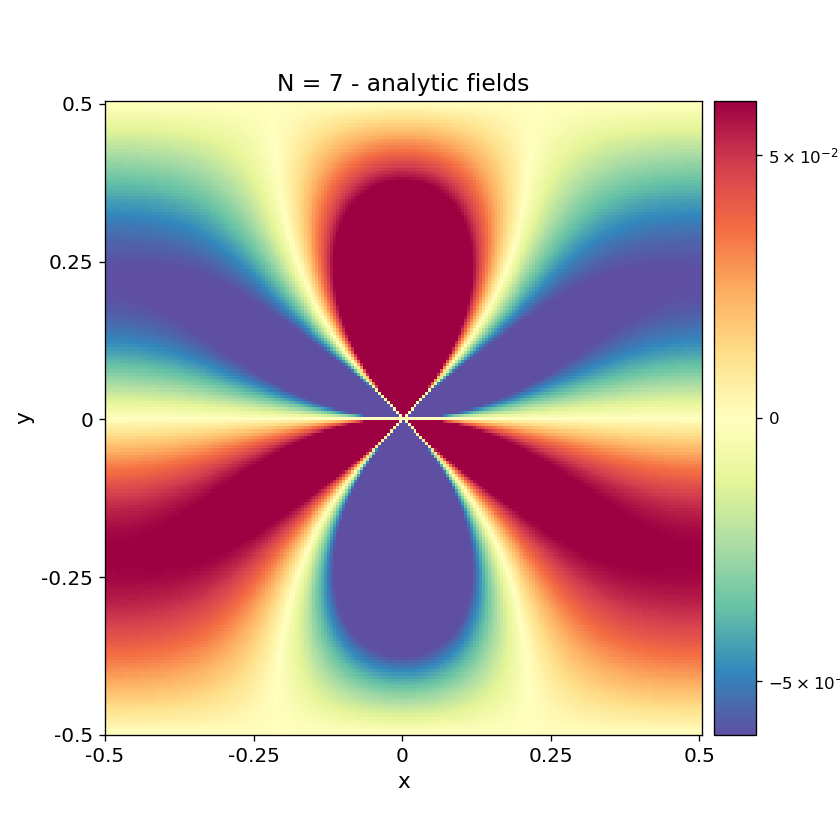
\includegraphics[width=0.7\textwidth]{../stress_field_07.png}
    \end{figure}
\end{frame}

\begin{frame}
    \frametitle{Plot 8}
    \begin{figure}[H]
        \centering
        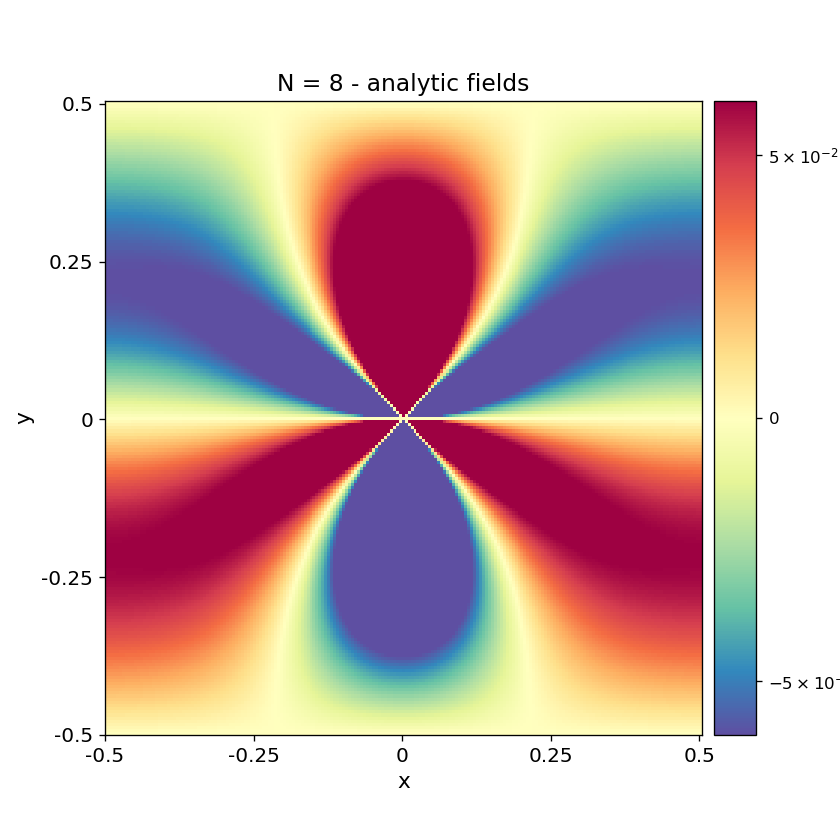
\includegraphics[width=0.7\textwidth]{../stress_field_08.png}
    \end{figure}
\end{frame}

\begin{frame}
    \frametitle{Plot 9}
    \begin{figure}[H]
        \centering
        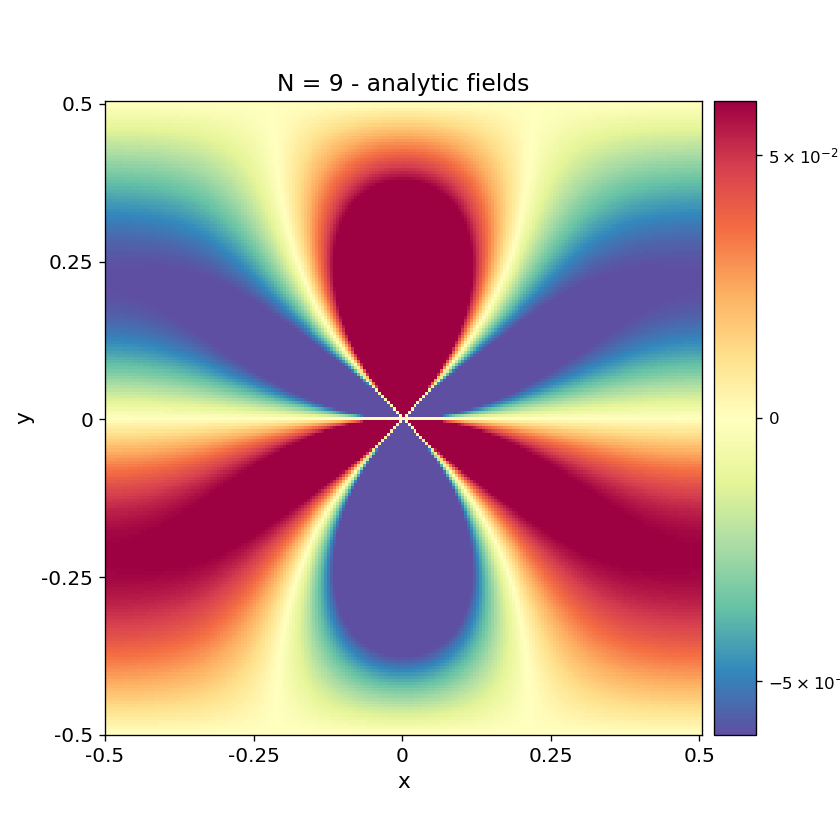
\includegraphics[width=0.7\textwidth]{../stress_field_09.png}
    \end{figure}
\end{frame}

\begin{frame}
    \frametitle{Plot 10}
    \begin{figure}[H]
        \centering
        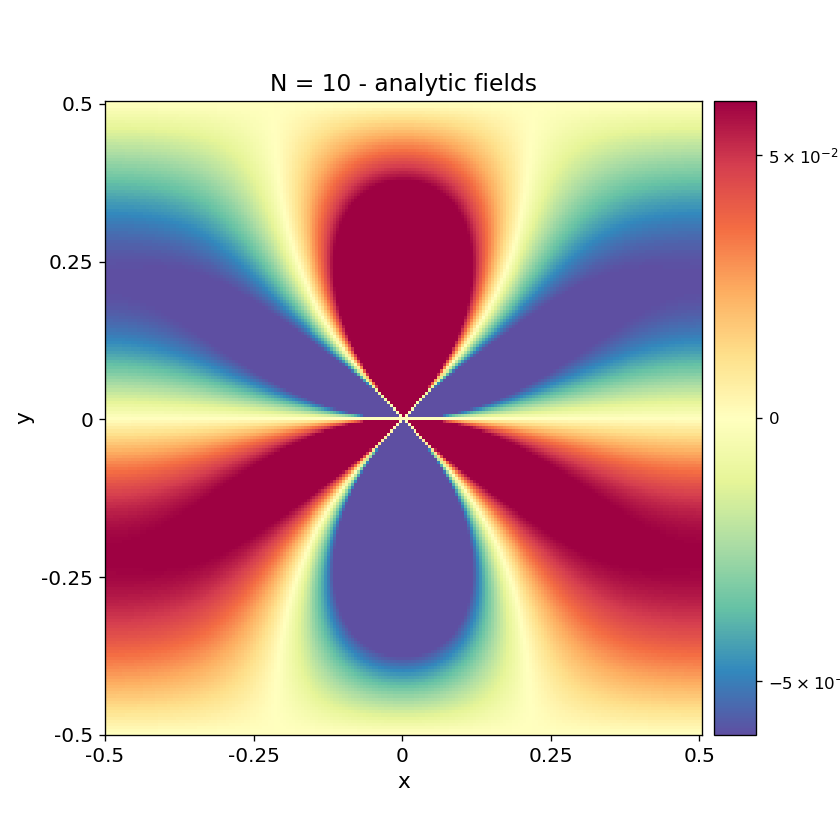
\includegraphics[width=0.7\textwidth]{../stress_field_10.png}
    \end{figure}
\end{frame}

\begin{frame}
    \frametitle{Plot 11}
    \begin{figure}[H]
        \centering
        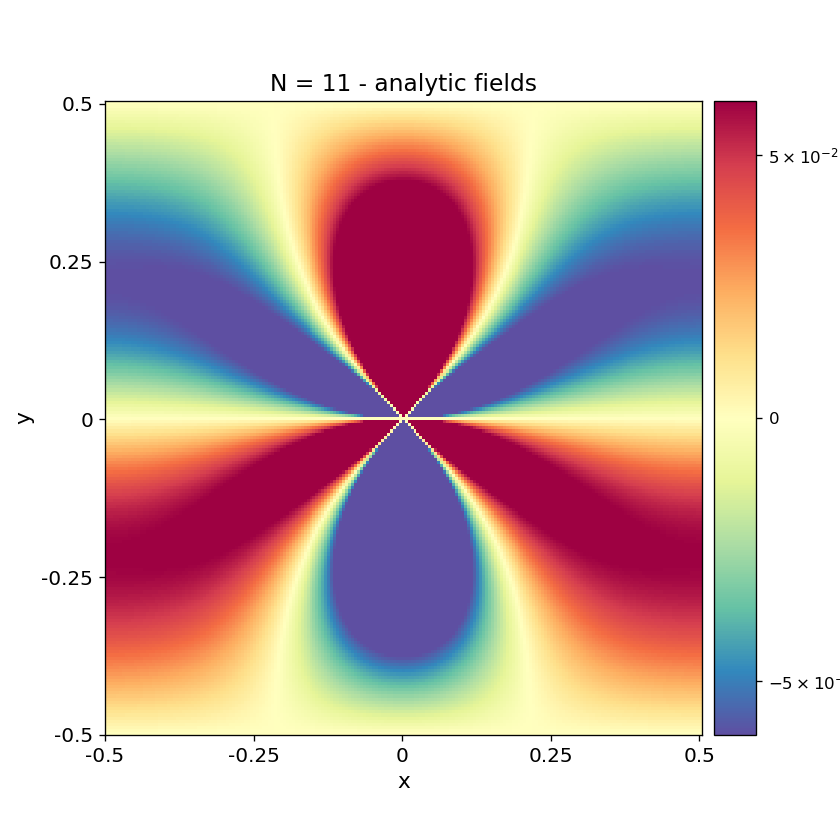
\includegraphics[width=0.7\textwidth]{../stress_field_11.png}
    \end{figure}
\end{frame}

\begin{frame}
    \frametitle{Plot 12}
    \begin{figure}[H]
        \centering
        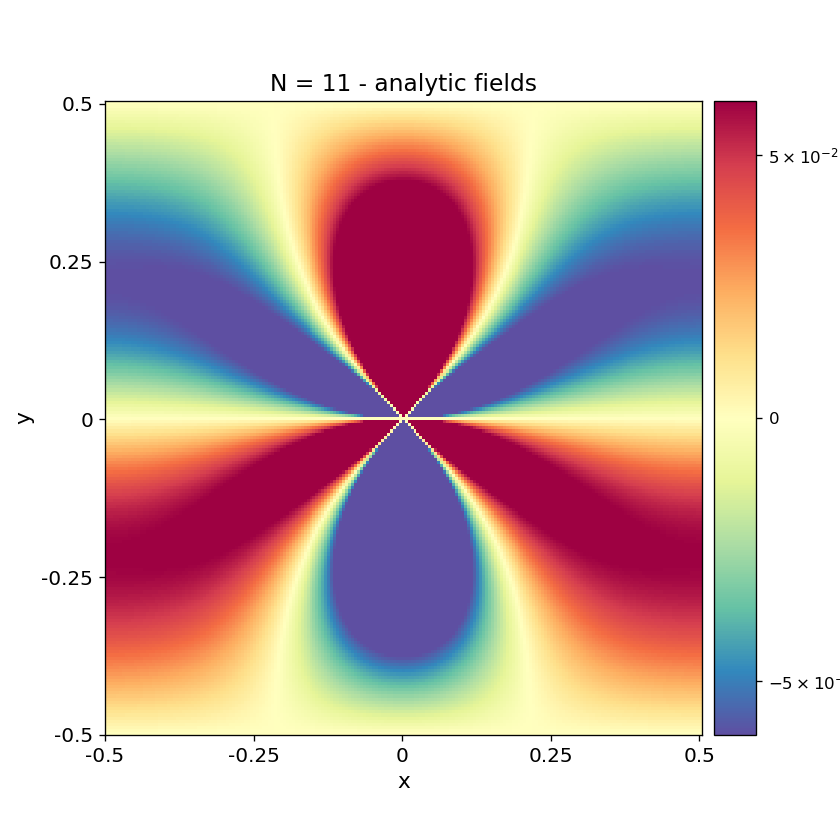
\includegraphics[width=0.7\textwidth]{../stress_field_11.png}
    \end{figure}
\end{frame}

%------------------------------------------------

\begin{frame}
    \frametitle{Difference of analytic fields}
    
    \begin{figure}[H]
        \centering
        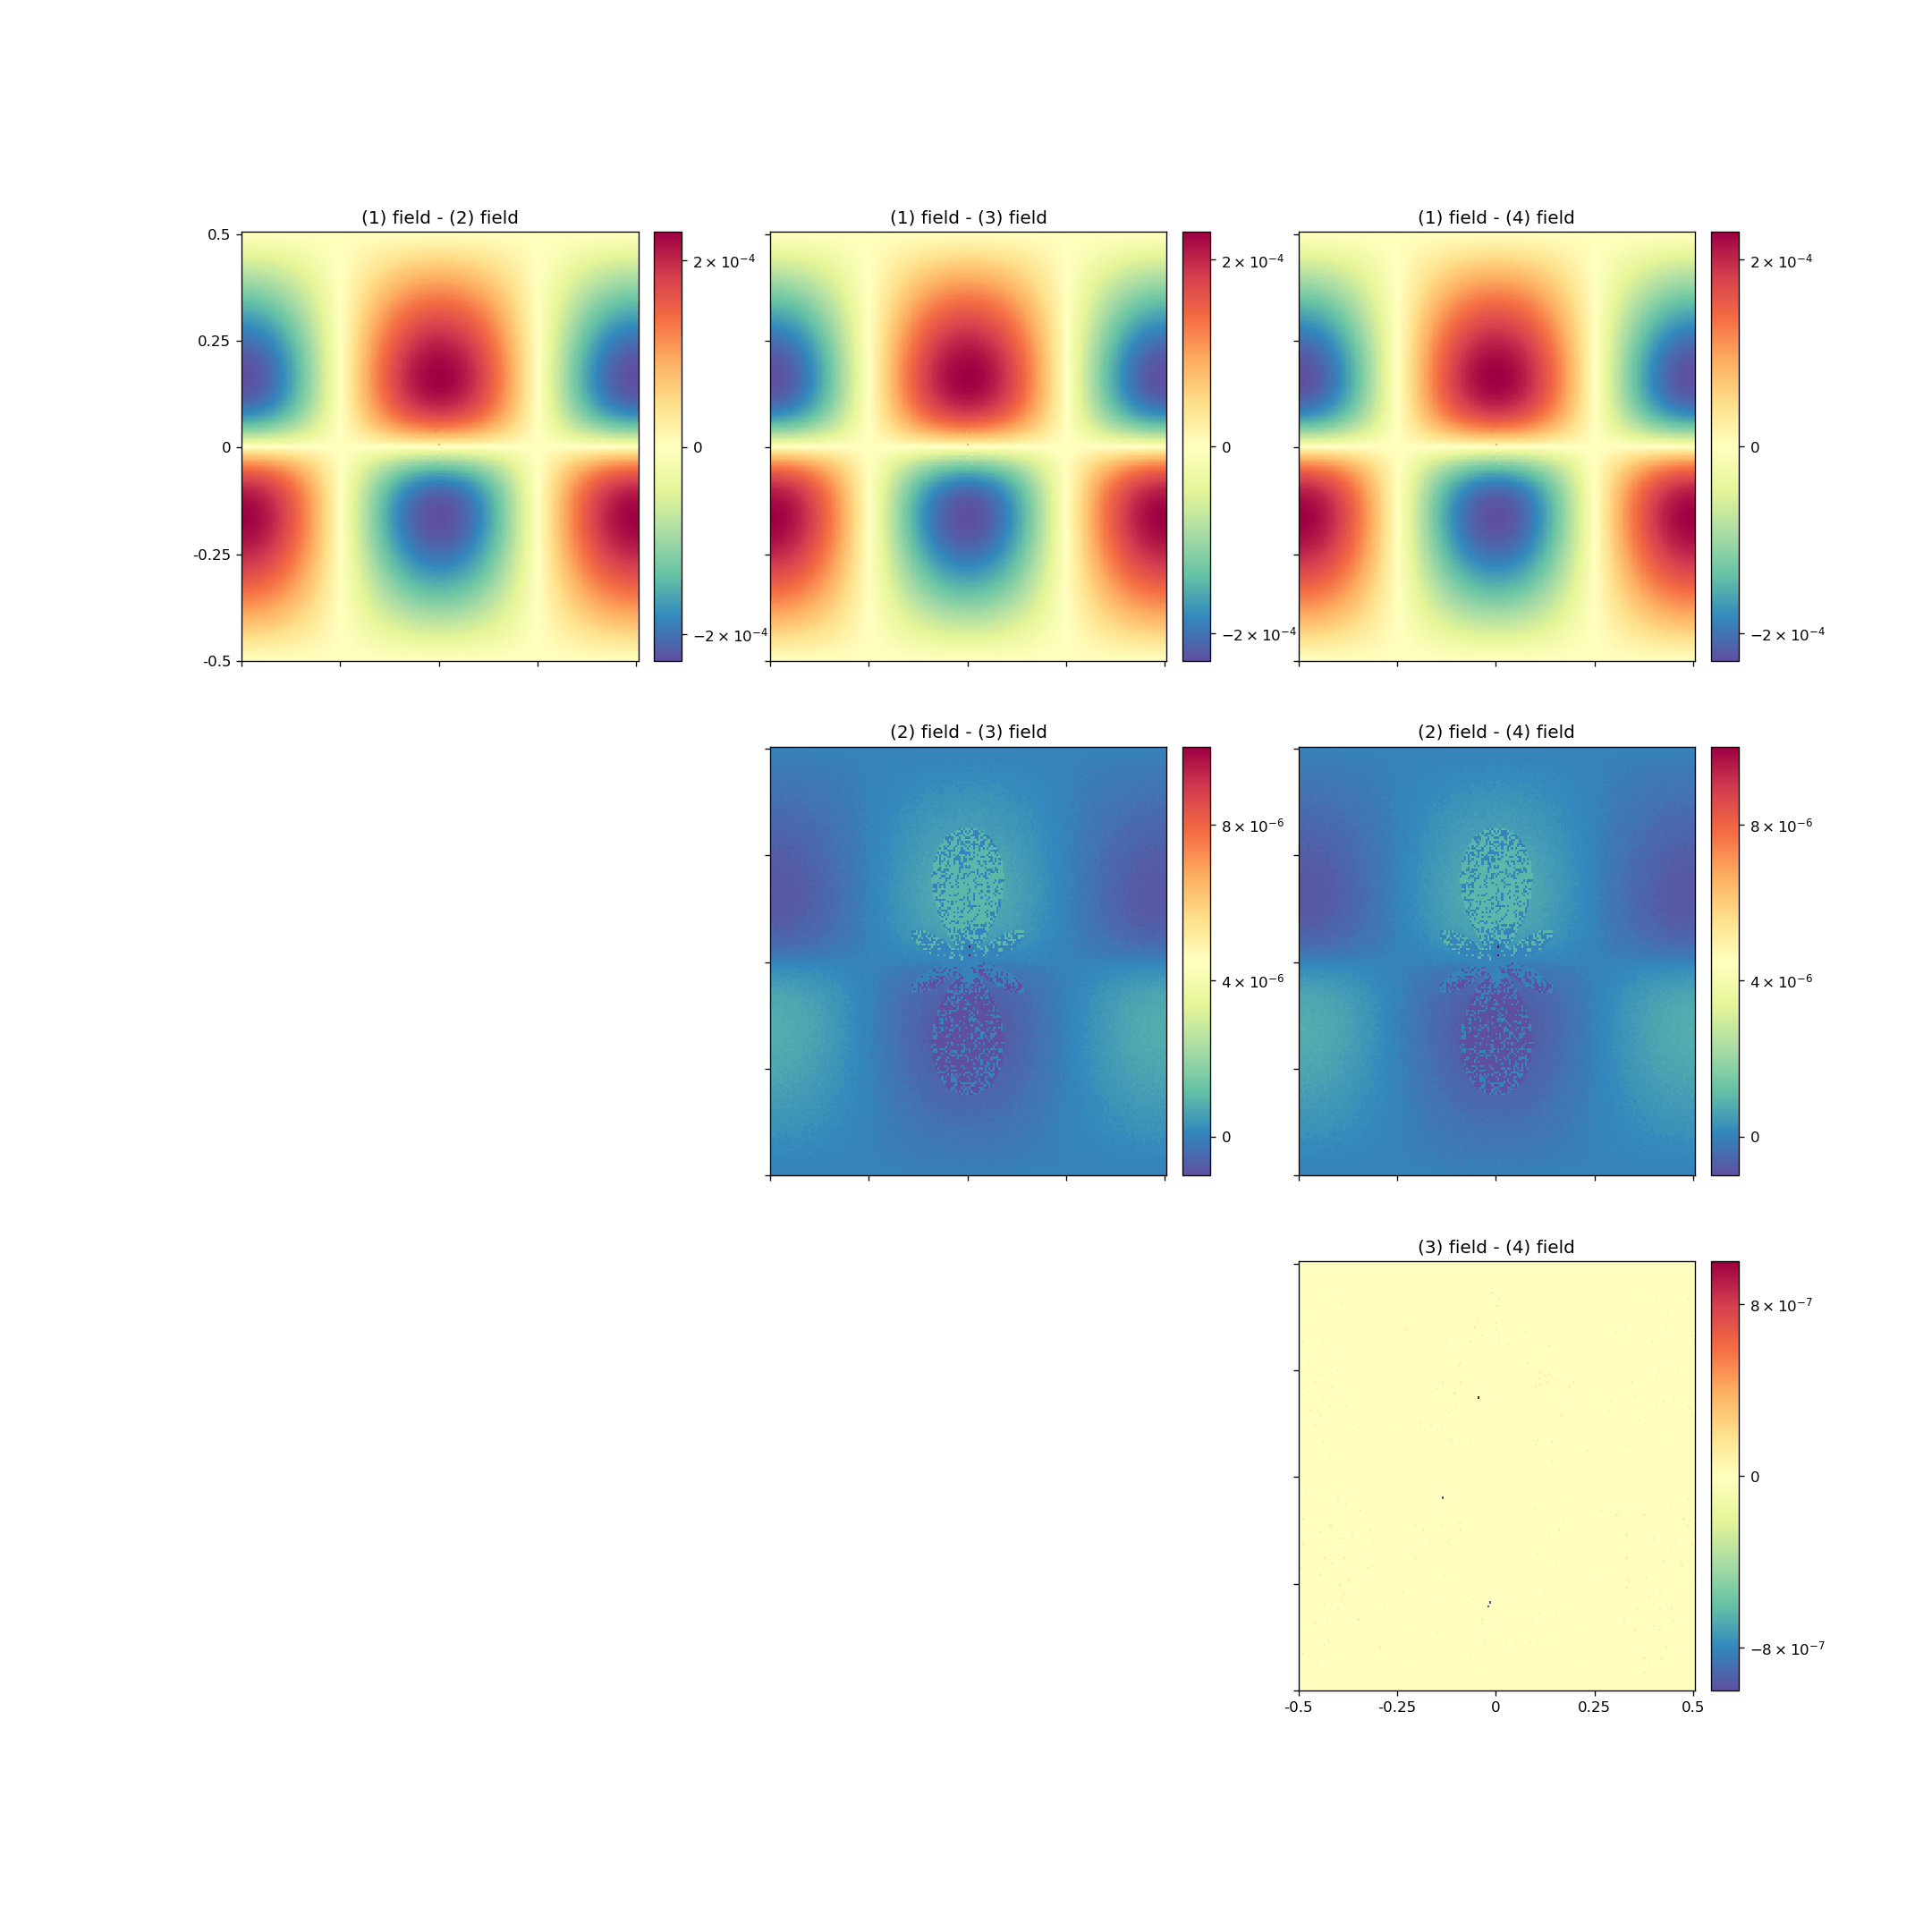
\includegraphics[width=0.825\textwidth]{../difference_of_analytic_fields.png}
    \end{figure}

\end{frame}

%------------------------------------------------

\begin{frame}
    \frametitle{ELTE stress field}
    
    \begin{figure}[H]
        \centering
        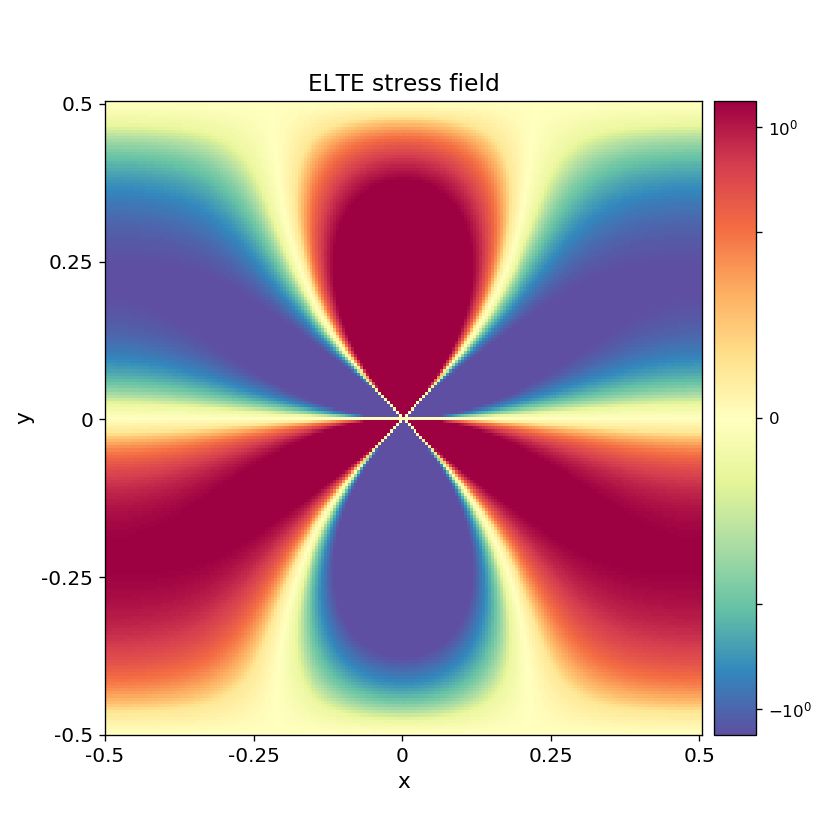
\includegraphics[width=0.825\textwidth]{../elte_stress_field.png}
    \end{figure}

\end{frame}

\begin{frame}
    \frametitle{Difference of analytic fields with ELTE field}
    
    \begin{figure}[H]
        \centering
        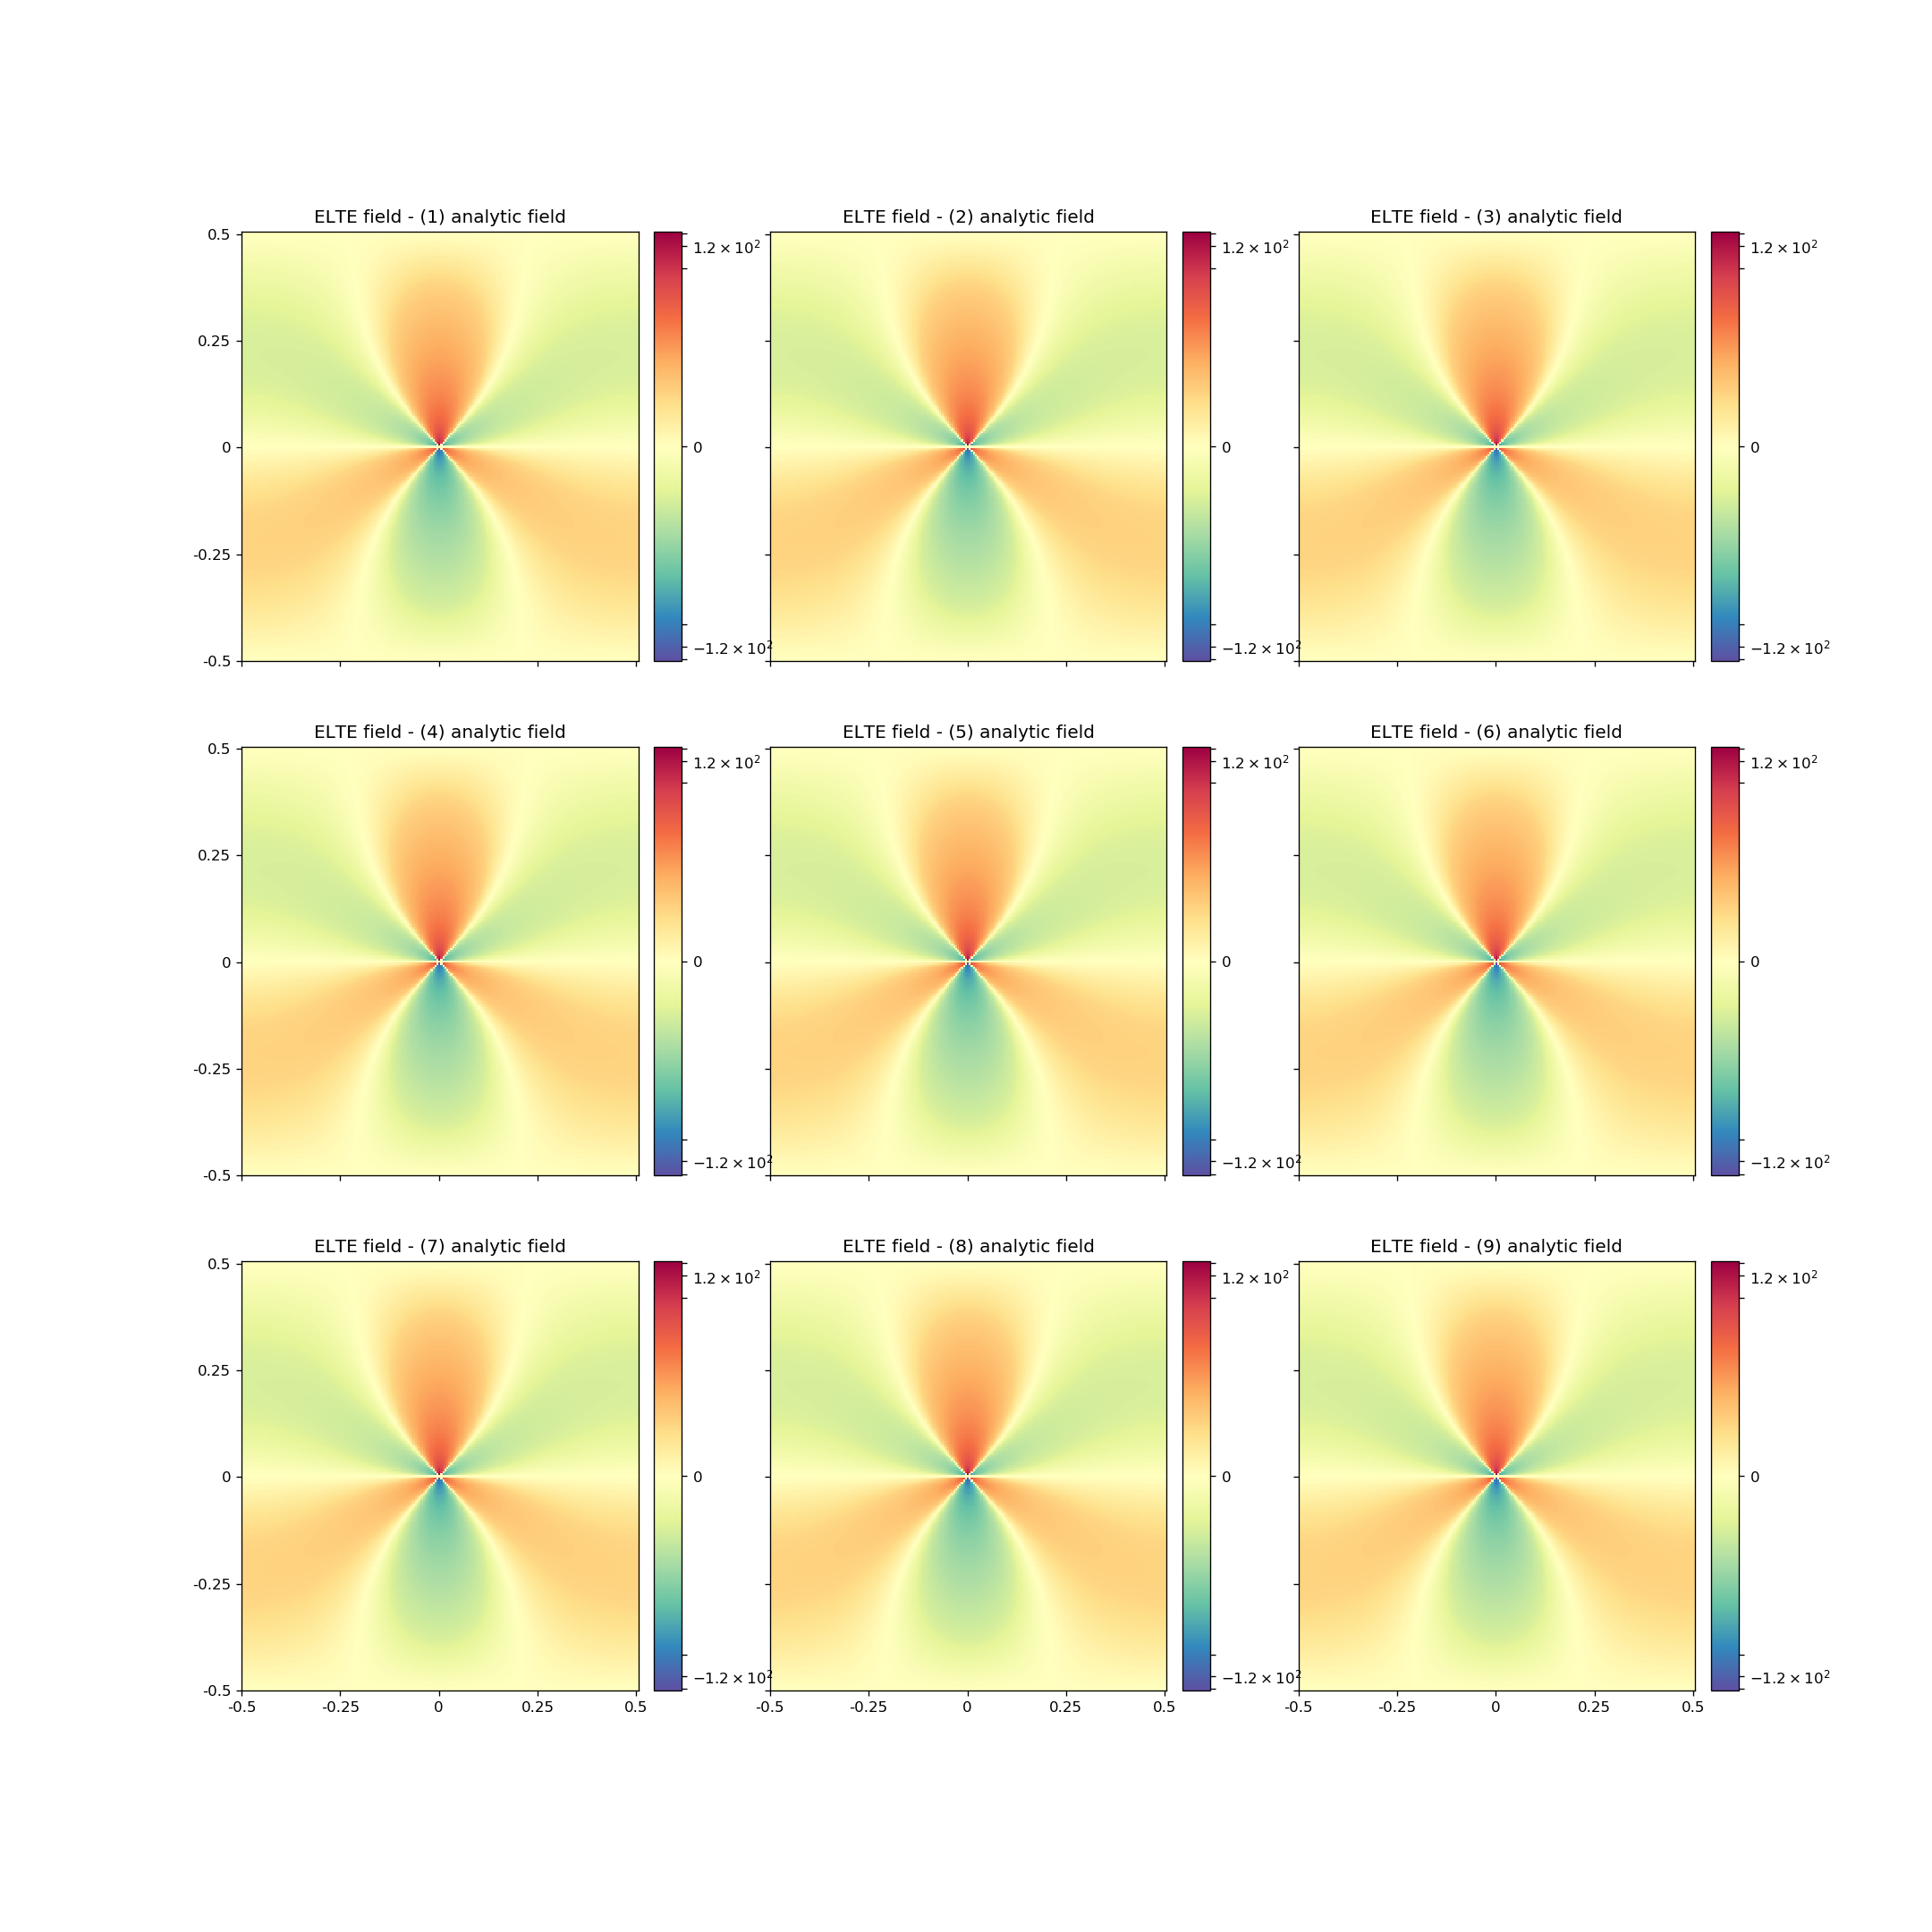
\includegraphics[width=0.825\textwidth]{../difference_of_analytic_field_and_elte_field.png}
    \end{figure}

\end{frame}

\begin{frame}
    \frametitle{Conclusion}
    
    \begin{itemize}
        \item considering N = 4 the analytic fields do not change significantly
        \item the difference with the ELTE stress field is most significant around the center
    \end{itemize}

\end{frame}

\end{document}